% Created 2013-03-02 Sat 22:35
\documentclass[11pt]{article}
\usepackage[utf8]{inputenc}
\usepackage[T1]{fontenc}
\usepackage{fixltx2e}
\usepackage{graphicx}
\usepackage{longtable}
\usepackage{float}
\usepackage{wrapfig}
\usepackage{soul}
\usepackage{textcomp}
\usepackage{marvosym}
\usepackage{wasysym}
\usepackage{latexsym}
\usepackage{amssymb}
\usepackage{hyperref}
\tolerance=1000
\DeclareUnicodeCharacter{22EE}{\vdots}
\author{G. Jay Kerns}
\date{March 2, 2013}
\title{Org-mode and \texttt{julia}: an introduction}
\hypersetup{
  pdfkeywords={},
  pdfsubject={},
  pdfcreator={Generated by Org mode 7.9.3f in Emacs 24.3.50.1.}}
\begin{document}

\maketitle
\tableofcontents

\newpage

This document is an introduction to Org-mode + \texttt{julia}. The only
prerequisites are a passing familiarity with Org-mode and Emacs
keybindings.

\section[What you need to get started]{What you need to get started}
\label{sec-1}

\textbf{Note:} several code blocks below have the header argument \texttt{:eval
  no-export}.  This means that the code block can be evaluated
  interactively by \texttt{C-c C-c} with point in the block but will \emph{not} be
  evaluated during export.  That header argument is present because
  those blocks have settings which conflict with my current setup (or
  are otherwise redundant) yet are meant to be useful for other
  people.

\subsection[Julia]{Julia}
\label{sec-1-1}

You are going to need a working installation of \texttt{julia}.  The homepage
on \href{https://github.com/JuliaLang/julia}{GitHub} has the pertinent links collected all in one place:

\begin{itemize}
\item \textbf{Homepage:} \url{http://julialang.org}
\item \textbf{Binaries:} \url{http://code.google.com/p/julialang/downloads/list}
\item \textbf{Packages:} \url{http://docs.julialang.org/en/latest/packages/packagelist/}
\item \textbf{Mailing lists:} \url{http://julialang.org/community/}
\item \textbf{IRC:} \url{http://webchat.freenode.net/?channels=julia}
\item \textbf{Source code:} \url{https://github.com/JuliaLang/julia}
\item \textbf{Git clone URL:} \texttt{git://github.com/JuliaLang/julia.git}
\item \textbf{Documentation:} \url{http://julialang.org/manual/}
\end{itemize}

\underline{Fair warning:} the initial install takes a \emph{long time}, largely
because julia has a lot of dependencies. Never fear, though;
subsequent updates are brief.
\subsection[ESS - Emacs Speaks Statistics]{ESS - Emacs Speaks Statistics}
\label{sec-1-2}

You are going to need a relavely bleeding-edge version of ESS since it
is only due to recent ESS changes that this document is even possible.
The place to look for the latest version of ESS is \href{http://stat.ethz.ch/ESS/index.php?Section=download}{here}.  At some
point after installation you will likely put something like the
following in your \texttt{.emacs}:

\begin{verbatim}
(require 'ess-site)
\end{verbatim}

Once ESS is up and running you will need to tell it where the \texttt{julia}
executable is. Edit the following and place it in your \texttt{.emacs}:

\begin{verbatim}
(setq  inferior-julia-program-name "/path/to/julia-release-basic")
\end{verbatim}

After the above steps are complete then you should be able to start
Emacs and launch an interactive \texttt{julia} session via \texttt{M-x julia}.  If
you manage to get that settled then at this point you should be able
to do everything in the \href{file://intro-julia.org}{Introduction to Julia}.
\subsection[Add-on packages]{Add-on packages}
\label{sec-1-3}

There is a growing list of \href{http://docs.julialang.org/en/release-0.1/packages/packagelist/}{contibuted packages} which add to the base
functionality of \texttt{julia}.  For example, several statistics packages
were mentioned a few moths ago in a blog post by \href{https://github.com/johnmyleswhite}{John Myles White}
entitled \href{http://www.johnmyleswhite.com/notebook/2012/12/02/the-state-of-statistics-in-julia/}{The State of Statistics in Julia}.  The instructions in the
blog post are (already) a bit out-of-date; the currently recommended
way to install the packages is to launch an interactive \texttt{julia}
session and execute the following command:

\begin{verbatim}
Pkg.add("DataFrames", "Distributions", "GLM", "MCMC", "Optim", 
        "NHST", "Clustering")
\end{verbatim}

I recommend you \textbf{not} execute the \texttt{Pkg.add} command here (if you do it
in this buffer then you can't watch the download and install as it is
happening).  As John notes, the \texttt{RDatasets} package takes a lot longer
to download than the others.  Perhaps it would be wise to install it
separately.

\begin{verbatim}
Pkg.add("RDatasets")
\end{verbatim}

You will notice both \texttt{Pkg.add} code blocks have the \texttt{:eval never}
header argument.
\subsection[Org-mode]{Org-mode}
\label{sec-1-4}

Since you have at least a passing familiarity with org-mode then you
probably already have something like the following in your \texttt{.emacs}:

\begin{verbatim}
(require 'org)
\end{verbatim}

Another handy setting to have is

\begin{verbatim}
(setq org-confirm-babel-evaluate nil)
\end{verbatim}

The following lines (either here or in your \texttt{.emacs}) permit inline
image display in the Emacs buffer.

\begin{verbatim}
(add-hook 'org-babel-after-execute-hook 'org-display-inline-images)   
(add-hook 'org-mode-hook 'org-display-inline-images)
\end{verbatim}
\subsection[\texttt{ob-julia.el}]{\texttt{ob-julia.el}}
\label{sec-1-5}

You are going to want a copy of \texttt{ob-julia.el} to fully integrate
\texttt{julia} with Org-mode.  You can find it and some other documents to
get you started \href{https://github.com/gjkerns/ob-julia}{here}.  Download \texttt{ob-julia.el} into a convenient place.
Edit the code block below and evaluate it by \texttt{C-c C-c} with point in
the code block.

\begin{verbatim}
(load "/path/to/ob-julia.el")
\end{verbatim}

An alternative method is to put the following in your \texttt{.emacs} (these
should go below the \texttt{(require 'org)} line):

\begin{verbatim}
(add-to-list 'load-path "/path/to/ob-julia.el")
(org-babel-do-load-languages
 'org-babel-load-languages
 '((emacs-lisp . t) (julia . t)))
\end{verbatim}

You are all set.
\section[Evaluation inside the Org buffer]{Evaluation inside the Org buffer}
\label{sec-2}

If you've gotten this far then everything is installed in the right
place and initialized properly. Now the fun begins.

\subsection[:results value]{:results value}
\label{sec-2-1}

The collection class of the \texttt{:results} header argument supports two mutually exclusive options: \texttt{value} and \texttt{output}.  When \texttt{:results value} is specified, Org takes the body of the source block, creates a function with that body, evaluates the function with \texttt{julia}, stores the result in a \texttt{.csv} file, then converts the \texttt{.csv} file to an \texttt{emacs-lisp} table, and finally inserts the table in the buffer.  \emph{Whew!}  The bottom line?  Hit \texttt{C-c C-c} in the following code block.

\begin{verbatim}
rand(2,3)
\end{verbatim}

\begin{center}
\begin{tabular}{rrr}
0.5584357754021063 & 0.9136408669454337 & 0.506642489779598\\
0.74985978094506 & 0.04938552792586104 & 0.596697983703395\\
\end{tabular}
\end{center}

As expected, the output of the command was a \texttt{2x3} array and Org inserted a table into the buffer.  This functionality is relatively powerful with other languages such as R, for instance, because \texttt{ob-R.el} works with \texttt{TAB} separated files instead and \texttt{read.table} in R supports reading of much more varied data types compared to \texttt{readcsv} in \texttt{julia} (at the present time).  Nevertheless, the functionality exists in \texttt{julia} and as time passes and \texttt{julia} adds more options we'll add more, too.  
\subsection[:results output]{:results output}
\label{sec-2-2}

We will get a lot more mileage out of the \texttt{:results output} option. Every command in the src block body is evaluated by \texttt{julia} in turn and the results are placed in the buffer to be typeset in a verbatim environment.  This option is similar to typing commands in \texttt{julia} at an interactive session.  The analogy isn't exact, though, because at an interactive session it is one (1) command in, one (1) result out.  Multiple lines in an org SRC block in contrast have RESULTS which are lumped together.  Like this: (do \texttt{C-c C-c})

\begin{verbatim}
2 + 3
print("hello")
sqrt(5)
\end{verbatim}

\begin{verbatim}
5
hello
2.23606797749979
\end{verbatim}

It is sometimes helpful to split up SRC blocks into smaller chunks so that buildup of RESULTS does not get out of hand.  Also, specific to \texttt{julia} we can sometimes put a semicolon at the end of the command to suppress output, like this:

\begin{verbatim}
2 + 3;
print("hello");
sqrt(5);
\end{verbatim}

\begin{verbatim}

hello
\end{verbatim}

Notice the outer two results were suppressed, but not the middle one.
\section[Graphics]{Graphics}
\label{sec-3}

The most stable and fully featured of the \texttt{julia} graphics packages at
the time of this writing appears to be the \href{https://github.com/nolta/Winston.jl}{Winston package}, although
the \href{https://github.com/dcjones/Gadfly.jl}{Gadfly package} is also available and appears promising.  To
install the Winston package execute the following in an interactive
session.  As above I recommend you \textbf{not} execute this here (hence the
\texttt{:eval never} header argument).

\begin{verbatim}
Pkg.add("Winston")
\end{verbatim}

The Winston package has lots of dependencies and many of them must be
built from source (on Ubuntu).

\subsection[Plotting with Winston]{Plotting with Winston}
\label{sec-3-1}

To get up and running with plots in \texttt{julia} check out the many example
graphs (with code) on the \href{https://github.com/nolta/Winston.jl/blob/master/doc/examples.md}{Winston examples page}. As far as Org-mode is
concerned, you can do plotting

\begin{enumerate}
\item Interactively with a plot window,
\item In-buffer with a \texttt{png},
\item Via export into \LaTeX{}, HTML, Beamer\ldots{}
\end{enumerate}

All three methods require setting up the plot object as a first step,
after, of course, loading the Winston package.  Let's set up a simple
plot object (do \texttt{C-c C-c} with point in the block):

\begin{verbatim}
using Winston
x = linspace(0, 3pi, 100)
c = cos(x)
s = sin(x)
p = FramedPlot();
setattr(p, "title", "title!")
setattr(p, "xlabel", L"\Sigma x^2_i")
setattr(p, "ylabel", L"\Theta_i")
add(p, FillBetween(x, c, x, s) )
add(p, Curve(x, c, "color", "red") )
add(p, Curve(x, s, "color", "blue") )
\end{verbatim}

We did \texttt{:results silent} to omit the lengthy output from being
inserted in the org buffer. So the hard part is finished -- we've
created a plot object \texttt{p} which is now available to manipulate.

To launch a plot window and look at the graph right now evaluate the
following code block.

\begin{verbatim}
Winston.tk(p)
\end{verbatim}

A plot should open in an X11 window with a pretty graph. Suppose
instead we'd like to insert the graph in the org buffer right now. We
need the inline-image display options described in section \texttt{Org
mode}. Assuming you've done that, evaluate the following code block.

\begin{verbatim}
file(p, "example1.png")
\end{verbatim}

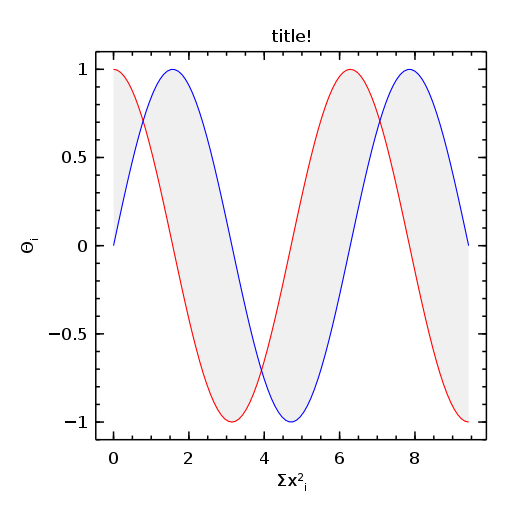
\includegraphics[width=.9\linewidth]{example1.png}

The code block evaluates the command \texttt{file(p, "example1.png")}, which
tells \texttt{julia} to write the graph to a \texttt{.png} file (also available are
\texttt{.pdf}, \texttt{.svg}, and \texttt{.eps}, though none of those can be inserted in
the org buffer).  The header argument \texttt{:results graphics} tells
org-mode that the results are going to be graphics (as opposed to
elisp tables or STDOUT output) and the header argument \texttt{:file
example1.png} tells org to insert an link to the file \texttt{example1.png}
(just created by \texttt{julia}) right after the the code block.  This link
is evaluated by \texttt{org-display-inline-images} which results in a \texttt{.png}
in the org buffer.

Notice that we had to specify the file name \emph{twice}, once inside the
code block and once as a header argument.  Some languages (such as R)
only require one specification: the header argument.  The reason for
this is simple: \texttt{ob-R.el} includes code which dynamically constructs a
graphics device call behind the scenes, the call depending on the file
extension in the \texttt{:file} header argument.  Such a thing is more
difficult with \texttt{julia} because different graphics packages have
markedly different device calls (for instance, \texttt{Gadfly} uses
\texttt{SVG("filename", p)}).  Maybe someday the calls will stabilize and it
will make sense to write wrapper code to do that automatically.  In
the meantime, use whatever package you like and write the filename
twice.

We'll defer the export method discussion to the next section.
\section[Export to other formats]{Export to other formats}
\label{sec-4}

Sooner or later you will want to share your work with others, people
who have not (yet) fully come to the realization that Emacs+Org is
really quite better than sliced bread and also is destined to conquer
the entire observable Universe.  Perhaps you'd like to make a
presentation about how awesome \texttt{julia} is at a(n) (inter)national
conference. Org-mode supports export to multiple formats.  Here we'll
describe a few.  There has been work recently on a brand new exporter
which hasn't yet made it to the official maintenance branch as of the
time of this writing.  The following instructions apply to the new
exporter, which is one of the reasons why it was important in the
first section to update your Org-mode.

\subsection[HTML]{HTML}
\label{sec-4-1}
This is the easiest. Insert the following in your \texttt{.emacs}:

\begin{verbatim}
(require 'ox-html)
\end{verbatim}

Then open this file and execute \texttt{C-c C-e} to open the export
dispatcher.  From there you have three options:

\begin{enumerate}
\item \texttt{h H} exports as an HTML buffer (can be saved later),
\item \texttt{h h} exports as an HTML file (saved in the working directory),
\item \texttt{h o} exports as an HTML file and opens in a browser.
\end{enumerate}

That's it.  There are a lot of other cool things you can do; see the
Org manual.  If you export to HTML then you are going to want your
images (if any) to be \texttt{.png} or \texttt{.svg} files.
\subsection[\LaTeX{}]{\LaTeX{}}
\label{sec-4-2}

This one is just as easy.  Insert the following in your \texttt{.emacs}:

\begin{verbatim}
(require 'ox-latex)
\end{verbatim}

Then open this file and do

\begin{enumerate}
\item \texttt{C-c C-e l L} to export as a \LaTeX{} buffer,
\item \texttt{C-c C-e l l} to export as a \LaTeX{} file,
\item \texttt{C-c C-e l p} to export as \LaTeX{} and generate a PDF,
\item \texttt{C-c C-e l o} to export as \LaTeX{}, generate PDF, and open.
\end{enumerate}

There are a \emph{ton} of other \LaTeX{} things to do.  See the Org manual.
If you export to PDF then it's fine to use image formats \texttt{.png},
\texttt{.eps}, or \texttt{.pdf}, but the \texttt{.png} exports as a blurry raster image -
use \texttt{.pdf} instead (or \texttt{.eps} for external plain \LaTeX{} export).
\subsection[Beamer]{Beamer}
\label{sec-4-3}

Beamer is a special case unto itself. The short story is that you need
the following in your \texttt{.emacs}:

\begin{verbatim}
(require 'ox-beamer)
\end{verbatim}

Then also add an entry for the beamer class in your \texttt{.emacs}.  Here is
a boilerplate version which you can customize to taste:

\begin{verbatim}
(add-to-list 'org-latex-classes
	     '("beamer"
	       "\\documentclass[presentation]{beamer}
        \[DEFAULT-PACKAGES]
        \[PACKAGES]
        \[EXTRA]"
	       ("\\section{%s}" . "\\section*{%s}")
	       ("\\subsection{%s}" . "\\subsection*{%s}")
	       ("\\subsubsection{%s}" . "\\subsubsection*{%s}")))
\end{verbatim}

Since beamer is such a special case I have tweaked a minimal \texttt{julia}
beamer presentation in \href{file://ob-julia-beamer.org}{Sample \texttt{julia} Presentation}. See there, see the
Org manual, and see Worg too for more information.
\section[Other things to mention]{Other things to mention}
\label{sec-5}

\begin{itemize}
\item You can extract all of the \texttt{julia} source code (also known as
\emph{tangling} the Org document) with the keystrokes \texttt{C-c C-v t}.  This
will generate a \texttt{julia} script (with extension \texttt{.jl}) in the working
directory.  Note that this capability is turned off by default.  You
can activate it by adding the header argument \texttt{:tangle yes} to those
code blocks you'd like to tangle or doing a buffer-wide header
setting with the line \texttt{\#+PROPERTY: tangle yes} near the top of the
org file.  See the Org manual for details.

\item At the time of this writing \texttt{ob-julia.el} only supports \texttt{:session}
evaluation and does not support external process evaluation. This
means that every \texttt{SRC julia} block should have a \texttt{:session
  SOMETHING} header argument.  Alternatively, you can put a
buffer-wide header argument at the top of the org file, something
like this:

\begin{verbatim}
#+PROPERTY: session *julia*
\end{verbatim}

\item You may have noticed that those \texttt{julia} code lines with no output
(for instance, lines with semicolons \texttt{;} at the end) generate an
empty line in the \texttt{\#+RESULTS} below the code block.  Consequently,
the first time you evaluate a \texttt{julia} code block without having
previously initiated a \texttt{julia} session with \texttt{M-x julia} the
\texttt{\#+RESULTS} will have an extra mystery empty line.  It is no
mystery.  The first statement executed by ESS when loading \texttt{julia}
is an \texttt{include} command.  That command has no output.  If that empty
line bothers you then execute the code block again; the mystery
empty line will disappear.

\item Be careful when executing code blocks with \texttt{:results value}.  Code
block evaluation in that case works by writing the \texttt{julia} commands
to an external file in the \texttt{/tmp} directory, evaluating the commands
with \texttt{julia}, writing the results to a comma-separated (\texttt{.csv})
file, then reading the \texttt{.csv} file and converting the result to
\texttt{elisp} for insertion to the org buffer.  Not all object types are
supported by \texttt{julia} for writing to \texttt{.csv} files, in particular,
\texttt{1x1} matrices and arrays of ASCII characters are not supported
(yet).  If you try to evaluate code blocks in those cases (or any
other case where output to \texttt{.csv} is not supported) then you will
get an error.

\item After playing around with \texttt{julia} for a while you will notice that
instead of printing long arrays it will elide them with vertical
dots in the middle of the output which look similar to this \(
  \vdots \) in the buffer.  It turns out that \LaTeX{} does not like
those three dots because they correspond to a special character, and
the upshot is that your org file will not export to \LaTeX{}
successfully.  One way around this is to explicitly declare that
special symbol in the \LaTeX{} header. That is the reason for the
following line at the top of this org file.

\begin{verbatim}
#+LaTeX_HEADER: \DeclareUnicodeCharacter{22EE}{\vdots}
\end{verbatim}

\item \texttt{ob-julia.el} does not support \texttt{rownames} and \texttt{colnames} like
  \texttt{ob-R.el} does.
\end{itemize}
% Generated by Org mode 7.9.3f in Emacs 24.3.50.1.
\end{document}